%%
%% Template intro.tex
%%

\chapter{Background}
\label{cha:back}

In this chapter, we define the social network Facebook central to this study, the source of our data set, notation used throughout 
this thesis, our choice of classification algorithms and our testing approach and methodology.

\section{Facebook}
\label{sec:data}

Facebook is the largest and most active social media service in the world (as of September 2012 it had more than 1 billion active users \cite{fbzise}).
Facebook users can create a profile containing personal preferences and information including their favourite music, favourite movies, 
inspirational people, interests, age, birthday, etc and have friendships and interactions between other users. 

The four main interactions between users are posts (posting something on a friends' wall), 
tags (being mentioned in a friends post or comment), comments (written data on a post) and likes (clicking a like button if a user 
likes a post or comment). The mediums for these interactions are across links (some URL), posts (some Facebook post), 
photos (some uploaded Facebook photo) and videos (some uploaded Facebook video).

Given the enormous scope of interaction and preference information available about each user, NICTA have developed an app capable of tracking 
and recording all pertinent user information. This app will be discussed in the following section.

%\cite{backstrom2011center} studied two types of user uses of Facebook, explicit communication interaction and viewing attention. Communication 
%is focused on a limited subset of friends whilst viewing attention is dispersed among a much larger set. This supports the approach of testing
%a wide array of user interactiuons and preferences, as each users preferences are driven by where their attention is focused.

\section{Data Set}
\label{sec:linkr}

NICTA developed a Facebook app named \emph{LinkR}. \footnote{The main developer of the LinkR Facebook App is Khoi-Nguyen Tran, a PhD student at the Australian National University.} 
This app collected information about users, their interactions and preferences as well as a subset of available information about 
their friends. The app tracked and stored this information for over 100 app users and their 39,000+ friends over a 4-month time period.

Exhaustive interaction and profile information could not be recorded for the app users friends and as such all analysis performed in this
thesis was carried out exclusively on app users for whom we have full interaction and profile data.

The table below summarises the interactions data collected from both app users and their friends which is used during our subsequent analysis.

\begin{table}[tbh!]
\centering
	\begin{tabular}{|l|r|r|r|r|} % cols: (left, center, right)
		\hline
		\textbf{App Users} & \textbf{Posts} & \textbf{Tags} & \textbf{Comments} & \textbf{Likes}  \\ \hline
		\textbf{Wall} & 36,539 & 7,711 & 18,266 & 15,999 \\ \hline
		\textbf{Link} & 5,304 & - & 5,757 & 6,566 \\ \hline
		\textbf{Photo} & 4,933 & 28,341 & 8,677 & 8,612 \\ \hline
		\textbf{Video} & 245 & 2,525 & 1,687 & 843 \\ \hline
		 \hline
		\textbf{App Users and Friends} & \textbf{Posts} & \textbf{Tags} & \textbf{Comments} & \textbf{Likes}  \\ \hline
		\textbf{Wall} & 4,301,306 & 1,215,382 & 3,122,019 & 1,887,497 \\ \hline
		\textbf{Link} & 678,612 & - & 693,930 & 995,214 \\ \hline
		\textbf{Photo} & 1,268,816 & 9,620,708 & 3,431,321 & 2,469,859 \\ \hline
		\textbf{Video} & 59,244 & 904,604 & 486,677 & 332,619 \\ \hline
	\end{tabular}
	\caption{Data records for interactions between users. Rows are the type of interaction, columns are the medium of interaction.}
	\label{tab:revpol}
\end{table}

\section{Notation}
\label{sec:notation}

The mathematical notation utilised during this thesis is outlined below.

\begin{itemize}
\item $N$ users $U$ with an $I$-element user feature vector $X$ where $X \in \mathbb{R}^I$ (alternatively if a second user is needed $Z \in \mathbb{R}^I$) 
and the length and components of $I$ are uniquely defined for each affinity feature.
\item A set of items $V$.
\item A friend function $Friend_{u,z}$ which is $True$ when users $u$ and $z$ are friends.
\item A liked function $Liked_{u,v}$ which is $True$ when user $u$ likes item $v$.
\item A relationship $R$ between users where $R_{i,u}$ is uniquely defined for each affinity feature.
\item An alters set $A$ for each user $u$ item $v$ pair, based on some relationship $R$ between other users $z$. 
Where $a_{u,v,r} = \{z | R_{u,z} \wedge Likes_{z,v}\}$.

\clearpage
This alters set can be visualised in the figure below:

\begin{figure}[tbh!]
	\begin{center}
		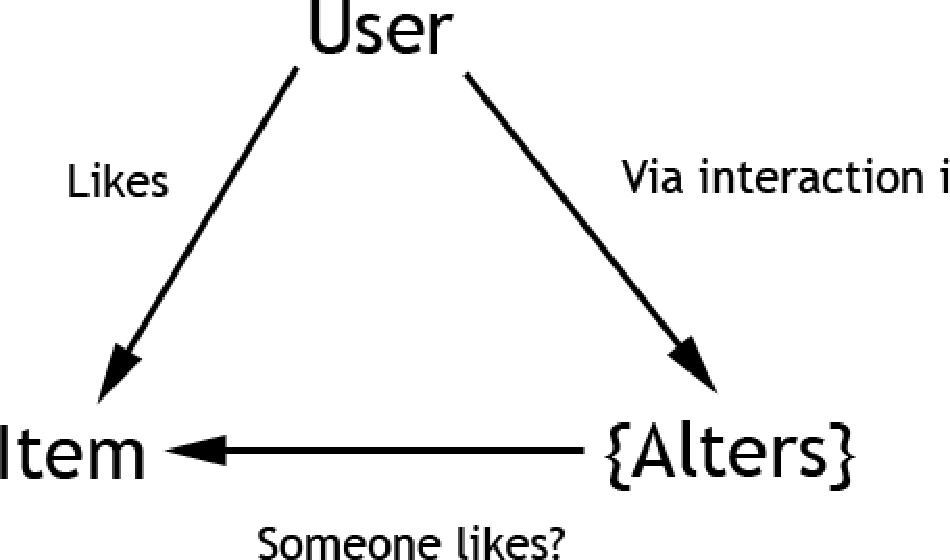
\includegraphics[scale=0.60]{imgs/alters.pdf}
		\caption{Alters paradigm. A user $u$ likes some item $m$, a relationship $R_{u,z}$ is defined via some affinity $i$ uniquely defined
		for each affinity feature, to create our set of alters $A$.}
	\end{center}
\end{figure}

\item An exposure $E$ where $E_{u,v,z} = \displaystyle\sum_{z}^{N} Friend_{u,z} \wedge Liked_{z,v}$ where this exposure can be 
limited by some $k$ with the condition $E_{u,v} >= k$.

This exposure can be visualised in the figure below:

\begin{figure}[tbh!]
	\begin{center}
		\includegraphics[scale=0.7]{results/imageLiked.png}
		\caption{Here we see an example of a link posted to a friends wall, which has subsequently been liked by two friends $z$. This 
				 demonstrates an exposure of $2$ for this link $m$.}
	\end{center}
\end{figure}

\item A data-set $D$ comprised of $D = \{(u,v,x) \to y\}$ where $u \in U$, $v \in V$ and the binary response $y \in \{0,1\}$ 
where $0$ represents a dislike and $1$ represents a like. 
\end{itemize}

\section{Affinity Features}
\label{sec:features}

Given the vast amount of potential affinity features available on Facebook, we need to break our features down into separate, distinct 
groups for testing purposes. Our two main groups will be \emph{user interactions} and \emph{user preferences}.

The individual components of these groups are displayed below:
\emph{User interactions}:
\begin{itemize}
\item \emph{Interactions} : Posts, Tags, Likes, Comments.
\item \emph{Outgoing Messages} : Messages sent to other users.
\item \emph{Incoming Messages} : Messages received from other users.
\end{itemize}

\emph{User preferences}:
\begin{itemize}
\item \emph{Demographics} : Age, Gender, Location.
\item \emph{Favourites} : Activities, Books, Athletes, Teams, Movies, Music, Sports, Television, Movies, People, Interests.
\item \emph{Groups} : All groups a user has joined.
\item \emph{Pages} :  All pages a user has liked.
\end{itemize}

Each of these affinity features will be discussed in detail under their separate sections of this thesis.
During our analysis we will compare the predictiveness of each of these affinity features individually, as well as in combination.

\section{Previous Work}
\label{sec:pw}

Two general approaches to prediction in a social context are \emph{content-based filtering} (CBF) \cite{newsweeder} which exploits 
item features based on items a user has previously liked and  \emph{collaborative filtering} (CF) 
\cite{collab_filtering} which exploits the current users preferences as well as those of other users. 

Previous work defined the term \emph{social} CF (SCF) \cite{joseph} which augments traditional CF methods with additional social 
network information, the results of this previous work and analysis using live user trials came to the conclusion that the approach of SMB
provided the best results for this data set and as such will be used as a baseline in this thesis.

These methods of CBF, CF and SCF result in a user gaining some similarity measure between other users, while the affinity features we 
explore during this thesis are based on explicit \emph{user interaction} and \emph{user preference} features and result in different 
models and predictions based on our choice of feature selection.

\section{Training and Testing}
\label{sec:tt}

All evaluation is applied using $10$ fold cross validation wherein the data is partitioned into $10$ complementary subsets, $80\%$ of 
these subsets are used for training while the remaining $20\%$ are used for testing.

The training and testing process is repeated $10$ times for each set of fold data. These results are then averaged to produce our 
estimates and standard error. The benefit of this method over repeated sub-sampling is all data points are used for both training 
and validation.

\section{Classification Algorithms}
\label{sec:meth}

Each classification algorithm used in this thesis is passed the training data for each fold as outlined above. The classifier 
builds a model representation of the data and applies this model to the test set to classify each test item into either a like or 
a dislike.

All affinity feature analysis carried out in this thesis will be performed on the following classification algorithms:

\subsection{Constant}
\label{sec:const}

The constant predictor returns a constant result irrespective of the feature vectors selected. Namely, this predictor returns $0$ (false)
regardless of the affinity feature represented by $X$. The most common result in our data set is $False$ and hence the $False$ 
predictor is displayed in all analysis, tables and graphs in this thesis.

\subsection{Social Match Box}
\label{sec:sr}

SMB is an extension of existing SCF techniques~\cite{lla,socinf} which constrain the latent space to enforce users 
who have similar preferences to maintain similar latent representations when they interact heavily.

SMB uses the social regularization method which incorporates user features to learn
similarities between users in the latent space which allows us to incorporate the social information of the Facebook data ~\cite{joseph}.

This objective component constrains users with a high similarity rating to have the same values in the latent feature space, which
models the assumption that users who are similar socially should also have similar preferences for items.

\subsection{Naive Bayes}
\label{sec:nb}

\emph{Naive Bayes} is a basic probabilistic classifier which involves applying Bayes' theorem using strong conditional independence 
assumptions between each feature in $X$. During training each element $i$ in the feature vector $X$ is devised to contribute some 
evidence that this $x_i$ belongs to either a like or dislike classification, during testing the class with the highest probability 
when applied to the model is the classification predicted. 

With feature vector $f \in \mathbb{R}^F$ derived from $(x,y) \in D$, denoted as $f_{x,y}$. NB learns a conditional model of the form 
$p(C|F_1, \dots, F_n)$ over a dependent class variable $C$ conditioned on the feature variables $F_1, \dots, F_n$. Applying both Bayes' rule 
and conditional independence assumptions the model can be rewritten as $p(C|F_1, \dots, F_n) = p(C) \displaystyle\prod_{i=1}^n p(F_i|C)$.

Classification of our test vector is achieved by choosing the most probable class of either like ($1$) or dislike ($0$).
\\
$\mathrm{classify}(f_1,\dots,f_n) = \underset{c \in \{1,0\}}{\operatorname{argmax}} \ p(C=c) \displaystyle\prod_{i=1}^n p(F_i=f_i\vert C=c)$.

\subsection{Logistic Regression}
\label{sec:lr}

\emph{Logistic Regression} directly estimates parameters based on the training data assuming a parametric form of the distribution.
LR predicts the odds of a feature vector $X$ being either a like or a dislike by converting a dependent variable and 
one or more continuous independent variable(s) into probability odds.

The probability $p_i$ is modelled using a linear predictor function $l(i)$, the linear predictor function of a particular point $d$ 
is written as $l(i) = \beta_0 + \beta_1 x_{1,i} + \cdots + \beta_M x_{m,i}$, where each data point $d$ is associated with an explanatory 
feature vector $X$ and $\beta_0, \ldots, \beta_M$ are regression co-efficients indicating the relative effect of a particular 
explanatory variable $x_{m,i}$ on the prediction.

The probability of a particular outcome is linked to the linear prediction function, 
$\operatorname{logit}(\mathbb{E}[Y_i|x_{1,i},\ldots,x_{m,i}]) = \operatorname{logit}(p_i)=\ln\left(\frac{p_i}{1-p_i}\right) = \beta_0 + \beta_1 x_{1,i} + \cdots + \beta_M x_{m,i}$
Where the class of either dislike ($0$) or like ($1$) with the higher probability is the prediction made.

The LR implementation used during this thesis is \emph{LingPipe} \cite{lin}.

\subsection{Support Vector Machine}
\label{sec:svm}

The \emph{Support Vector Machine} is a supervised learning machine based on a set of basis functions which help construct 
a separating hyperplane between data points. Training involves building the relevant hyperplanes which can then be used for testing. 
Each data point is classified as a like or dislike depending on which side of the hyperplane it falls.

With feature vector $f \in \mathbb{R}^F$ derived from $(x,y) \in D$, denoted as $f_{x,y}$. A linear SVM learns a weight vector $w \in \mathbb{R}^F$
such that $w^T f_{x,y} > 0$ indicates a like classification of $f_{x,y}$ and $w^T f_{x,y} \leq 0$ indicates a dislike classification.

The SVM implementation used during this thesis is \emph{SVMLibLinear} \cite{cjlin}.

\section{Evaluation Metrics}
\label{sec:notation}

When evaluating the success of each affinity feature at correctly classifying an item, the following metrics have been analysed.

\begin{itemize}
\item A \emph{true positive} (TP) prediction refers to when the prediction correctly identifies the class as true. 
\item A \emph{false positive} (FP) occurs when the prediction is true, but the true class was false.
\item A \emph{false negative} (FN) occurs when the prediction is false but the actual class is true.
\end{itemize}

These definitions can be visualised using the table below. Where:
\\
$y$ represents the true class value $y \in \{0,1\} : actual$
\\
$\hat{y}$ represents the class prediction $\hat{y} \in \{0,1\} : prediction$.

\begin{table}[tbh!]
\centering
\begin{tabular}{r|l|l|l|}
\multicolumn{1}{r}{}
 &  \multicolumn{3}{c}{$y$} \\
 \cline{2-4}
& & \textbf{T} & \textbf{F} \\ 
\cline{2-4}
$\hat{y}$ & \textbf{T} & TP & FP \\
\cline{2-4}
& \textbf{F} & FN & TN \\
\cline{2-4}
\end{tabular}
\caption{Actual and prediction comparison table.}
	\label{tab:revpol}
\end{table}

Accuracy relates to the closeness to the true value. In the context of our results, the accuracy refers to the number of correct classifications 
divided by the size of the data set.

\[ \text{accuracy} = \frac{\text{number of correct classifications}}{\text{size of the test data set}}\]

Precision relates to the number of retrieved predictions which are relevant. In the context of our results, the precision refers to the number of TP predictions 
divided by the sum of the TP and FP predictions.

\[ \text{precision} = \frac{\text{number of TP}}{\text{number of TP + number of FP}}\]

Recall refers to the number of relevant predictions that are retrieved. In the context of our results, recall refers to the number of TP predictions 
divided by the sum of the TP and FN predictions.

\[ \text{recall} = \frac{\text{number of TP}}{\text{number of TP + number of FN}}\]

The f-score combines and balances both precision and recall and is interpreted as the weighted average of both precision and recall. 

\[ \text{f-score} = 2 \times \frac{\text{precision} \times \text{recall}}{\text{precision} + \text{recall}}\]

The main metric we use for analysis, tabulation and graphing in this thesis is accuracy.

%%% Local Variables: 
%%% mode: latex
%%% TeX-master: "thesis"
%%% End: 
